\section{Theory}\label{sec:Theory}

\newcommand{\state}{\ket{\psi}}
\newcommand{\hoket}{\ket{\phi}}
\newcommand{\hoep}{\ket{\phi +}}
\newcommand{\hoem}{\ket{\phi -}}
\newcommand{\pin}{\psi_\text{in}}
\newcommand{\pout}{\psi_\text{out}}
\newcommand{\kpin}{\ket{\psi_\text{in}}}
\newcommand{\kpout}{\ket{\psi_\text{out}}}
\newcommand{\mop}{\Omega_{+}}
\newcommand{\mom}{\Omega_{-}}
\newcommand{\melt}[3]{\left|\mel{#1}{#2}{#3}\right|^{2}}
\newcommand{\scat}{\mathcal{S}}
\newcommand{\mscat}{\(\scat\)}
\newcommand{\oop}[1]{\mathcal{#1}}
\newcommand{\moop}[1]{\(\oop{#1}\)}
\renewcommand{\vu}[1]{\mathbf{\hat{\text{$#1$}}}}

\subsection{Quantum Chromo-Dynamics}

Quantum chromo-dynamics is the base on which our modern understanding of the
nuclear force stands, but it cannot itself be used to model the nuclear force
by any practical means. This is due to its unperturbative nature at low energies, the energy regime of
nuclear interactions. The problem remained intractable until Weinberg in
1979 developed the concept of effective field theories (EFT)\cite{Weinberg1979}.

The underlying idea of EFT is reminiscent of multipole expansion in
electromagnetic field
theory. The complex short-range interactions of an electromagnetic field can be
approximated by a simpler structure when one is only concerned about the long
range interaction, such as treating an arbitrary charge distribution as a point
charge at large distances. Perhaps the most advantageous property of an EFT is
that a bound on the resulting approximation error can be systematically
established and improved, akin to including more multipoles and computing the
order of the truncation.

Chiral perturbation theory (ChPT) is an EFT of QCD built upon the symmetries relevant
in the nuclear energy regime allowing for a systematic treatment of the model
errors. Instead of having quarks and gluons as the degrees of freedom as they
are in QFT, the
effective degrees of freedom become the nucleons and pions. More energetic
phenomena like nuclear
resonances and mesons are integrated out\cite[p.~11]{EPELBAUM2012343}. This leads to ChPT's
inability to model such phenomena, and might be taken as an argument against it.
However, the model's inability to account for higher energy interactions does
not invariably lead to failure to explain low energy interactions. As argued by Ken
Wilson, it is better to admit that the high energy physics are unknown and treat
it as such. Since there are many high energy extensions consistent with a low energy
model, there is no need to pick the most ``realistic'' model, only the most practical.

There are several ways to develop an EFT for the nuclear regime. The majority of
modern nuclear EFTs are based on chiral symmetry, using the approach outlined by Weinberg in
1979 and expanded upon in 1990\cite{WEINBERG19913}. The Lagrangian used is the most general possible while being
constrained by chiral and additional symmetries\footnote{The
  curious reader might wonder why chiral symmetry has such a central role in
  nuclear low energy phenomena. As far as I know, besides the normal QCD arguments of symmetries and
  Goldstone bosons, there is no intuitive explanation for the connection between
  chirality and nuclear interactions.}. From the resulting infinite
amount of terms, a finite number is selected through perturbative expansion. The
details are technically complicated and surprisingly unenlightening. Only a short high level overview will be
given in the following paragraphs. More details are available in a plethora of
write-ups, such as \cite{EPELBAUM2012343,MACHLEIDT20111,lepage1997renormalize}.


To perform a perturbative expansion it is necessary to identify separation of
scales. For ChPT there are two scales: a soft scale \(Q\) being the external
momenta or the pion mass \mbox{\(m_{\pi} \approx \SI{140}{MeV}\)}, and a hard
scale\footnote{The value of the hard scale \(\Lambda_{\chi}\) is unknown, but is
bounded above by \mbox{\(4\pi F_{\pi}\approx \SI{1200}{MeV}\)}\cite[p.~18]{EPELBAUM2012343} and below by the first
non-Goldstone meson \(\rho\), \(m_{\rho}\approx \SI{770}{MeV}\). Picking a value
in the range \mbox{\(500-1000\) MeV} is a common choice for
calculations\cite[p.~29]{lepage1997renormalize}.
Others suggest going so low as \SI{300}{MeV}\cite[p.~64,p.~36]{dickhoff2008many,lepage1997renormalize}.}
\(\Lambda_{\chi}\sim \SI{1}{GeV}\), also called the symmetry breaking scale or
hadronic scale. The expansion is performed in powers of \(\left(
  Q/\Lambda_{\chi} \right)^{\nu}\), where \(\nu\) is known as the \textit{chiral
order}.

The ChPT Lagrangian can be separated into terms for different interactions,
\begin{equation*}
  \label{eq:1}
  \mathcal{L}_{\text{eff}} = \mathcal{L}_{\pi\pi} + \mathcal{L}_{\pi N} + \mathcal{L}_{NN}+\ldots ,
\end{equation*}
where \(\mathcal{L}_{\pi\pi}\) is pionic dynamics, \(\mathcal{L}_{\pi N}\)
is interactions between pions and a nucleon, and \(\mathcal{L}_{NN}\) the
contact\footnote{An interaction modeled by having no force carrier is a
  \textit{contact} interaction, having a special place due to its mathematical simplicity.} interactions between two nucleons. The ellipsis denotes higher order
interactions, such as the interaction of pions and two nucleons
\(\mathcal{L}_{\pi NN}\). Each of these terms
contains in turn an infinite amount of terms. 
The choice of which terms to include in our effective theory is done through a
rather technical scheme whereby one assigns a chiral order to all associated
Feynman diagrams and selects a highest order \(\nu\geq 0\). The number of terms
associated with a particular \(\nu\) is guaranteed to be finite, and the error
from ignoring all higher order diagrams is bounded by \(\left(
  Q/\Lambda_{\chi} \right)^{\nu+1}\). 

From \(\nu=0\) we obtain the lowest, or leading, order (LO). It is rather crude
with only two NN contact terms, but already accounts for the tensor force,
necessary to describe the deuteron\cite[p.~18]{Machleidt_2011}. Partial waves of very high angular
momentum are adequately described, while \(S\)-waves are only roughly correct up
to medium range. \(\nu=1\) vanishes, meaning the next-to-leading order (NLO)
has \(\nu=2\). This order includes central, spin-spin, spin-orbit and tensor
terms; all spin-isospin structures necessary to describe the two-nucleon force
phenomenologically. The intermediate-range interaction is not yet well described.
It is known\cite{MACHLEIDT19871,PhysRevC.21.861} that \(\Delta (1232)\)-isobar contributions are necessary for
a good description of the nuclear force, and these are introduced in \(\nu=3\),
the next-to-next-to-leading order (NNLO). \(\nu=4\) (N\(^{3}\)LO) is currently the highest
order which is computationally feasible, but  is not of interest to us here due
to its complexity.

There is undoubtedly a lot of work involved in creating an EFT potential.
Is this really necessary, one may wonder, why not use a phenomenological potential
instead? It is important to realize that EFT is
not glorified curve fitting. When a term is added to a phenomenologically motivated potential
trying to account for some high energy discrepancy, high energy data is required
to improve the fit, and the majority of the improvement will lie at high
energies. In contrast, adding a higher order term to an EFT potential gives a
better fit for all energies, and requires only low energy data to perform the
fit.  It is a method guaranteed to systematically improve the
solution, where loss of improvement hints at as of yet unknown physics. 

%The quantum field theory developed in the 1930s and 1940s had
% The formalism of computing Feynman diagrams led to difficulties when working
% with loops. Infinities pop up left, right and center, giving nonsensical
% results. A formalism was developed by Feynman, Schwinger, Tomonaga and Dyson [ref] to nevertheless obtain sensible values
% through systematically canceling infinities. Despite the impressive agreement with
% experiments [ref], many [who?] felt icky about the method, afraid it was nothing
% more but a mathematical trick, and our failure to understand it implied a
% failure to understand the physical significance.

% It wasn't before 1970s[when?] that Ken Wilson, an otherwise unknown physicist,
% illuminated the issue [ref]. The loop diagrams gave infinities because one has to sum
% over all possible [diagrams. clumsy structure, rewrite], for all energies. However, we do not know
% that QFT is the correct theory for high energy physics, nor is it necessary to
% assume so in order to do calculations at lower energies. One can instead set an
% arbitrary[not practically arbitrary, make clearer] limit \(\Lambda\) above which
% is the high energy, or \textit{ultraviolet} (UV), regime, and below which is the low
% energy, or \textit{infrared} (IR), regime [det ble nøstes. nøst opp]. Ken Wilson
% argued it is better we admit the physics of UV is unknown and treat it as such,
% and instead develop a low energy model. That the physics of UV is irrelevant can
% be seen from the fact that any low energy model has many consistent high energy
% models, or \textit{completions} [ref]. This gave rise to \textit{effective field
%   theories} (EFT).

% A more or less general procedure was developed to generate an EFT\cite[p.~7]{Machleidt_2011}:
% \begin{enumerate}
% \item  Identify the soft and hard scales, and the degrees of freedom appropriate
%   for (low-energy) nuclear physics.
% \item Identify the relevant symmetries of low-energy QCD and investigate if and how they are broken.
% \item Construct the most general Lagrangian consistent with those symmetries and symmetry breakings.
% \item Design an organizational scheme that can distinguish between more and less important contributions:
%   a low-momentum expansion.
% \item Guided by the expansion, calculate Feynman diagrams for the problem under consideration to the
%   desired accuracy.
% \end{enumerate}
% [seems out of place, as all steps except 5. are intractable by me]

% \subsection{The Chiral Lagrangian}

% In QCD the Lagrangian is\cite[p.~7]{Machleidt_2011}

% \begin{equation*}
%   \mathcal{L}_{\text{QCD}} = \bar{q}(i\gamma^{\mu}\mathcal{D}_{\mu} - \mathcal{M})q
%   - \frac{1}{4}\mathcal{G}_{\mu\nu,a}\mathcal{G}^{\mu\nu}_{a}
% \end{equation*}
% with \(\mathcal{D}_{\mu} = \partial_{\mu} - i
% g\frac{\lambda_{a}}{2}\mathcal{A_{\mu},a}\) the gauge-covariant derivative,
% \(\mathcal{G}_{\mu\nu,a}\) the gluon field strength tensor, \(q\) the quark
% fields and \(\mathcal{M}\) the quark mass matrix.

% [vanishing quark mass]

% [short about chiral symmetry]

% [explicit and spontaneous symmetry breaking]

% [chiral effective Lagrangian]


% In QCD the u  and d quarks have approximately chiral symmetry.
% Explicelty broken because u and d do not have the same mass
% Spontaneously broken

% Rekkeutvikling av Lpipi

% Chiral order

\subsection{The EFT Potentials}

After the brief overview of how to derive nuclear potentials from EFT, it is
time to present the results. The general form of the LO, NLO and NNLO potentials is\cite[p.~30-36]{Machleidt_2011}.
\newcommand{\greyout}[1]{{\textcolor{gray}{#1}}}
\begin{align}
  V^{LO} &= V^{(0)}_{\text{ct}}+V_{1\pi}\\
  V^{NLO} &= V_{LO} + V_{\text{ct}}^{(2)} \greyout{+ V_{2\pi}^{(2)}}\\
  V^{NNLO} &= V_{NLO} \greyout{+ V_{2\pi}^{(3)}},
\end{align}
where \(V^{(n)}_{\text{ct}}\) denotes contact terms of chiral order \(n\), and
\(V^{(m)}_{k\pi}\) denotes \(k\)-pion exchange terms with chiral order \(m\).
The greyed-out pion exchange terms are excluded in our toy potentials.
The contact terms are long and terribly unexciting. For the partial wave
\(^{1}S_{0}\) they reduce to simply

\newcommand{\pso}[0]{{\prescript{1}{}{S_{0}}}}
\newcommand{\pp}[0]{q}%{{p^{\prime}}}
\begin{align}
  \label{eq:contactterms}
  V^{LO}_{ct,\pso}(p, \pp) &= C_{0}\\
  V^{NLO}_{ct,\pso}(p, \pp) &= C_{2}(p^{2}+\pp^{2})\\
  V^{NNLO}_{ct,\pso}(p, \pp) &= C_{4}(p^{4}+\pp^{4}) + C_{4}^{\prime}p^{2}\pp^{2}.
\end{align}
The coefficients \(C_{0}, C_{2}, C_{4}, C_{4}^{\prime}\) are the model
parameters or \textit{low energy coefficients} (LECs).  There exists theoretical values for the coefficients, but due the truncation
and the ensuing renormalization, the values are rather useless. They
are instead obtained by fitting to data.


The full one-pion exchange term has the form
\begin{equation*}
  V_{1\pi}(\vec{p}, \vec{p}^{\prime}) = -\frac{g_{A}^{2}}{4f_{\pi}^{2}}\pmb{\tau}_{1}\cdot\pmb{\tau}_{2}
  \frac{\vec{\sigma}_{1}\cdot\vec{q}\vec{\sigma}_{2}\cdot\vec{q}}{q^{2}+m_{\pi}^{2}},
\end{equation*}
or in position space\cite[p.~30]{lepage1997renormalize}:
\begin{equation}
  \label{eq:onepion}
  V_{1\pi}(r) = \alpha_{\pi}\pmb{\tau}\cdot\pmb{\tau}\frac{\pmb{\sigma}_{1}\cdot\pmb{\nabla}\pmb{\sigma}_{2}\cdot\pmb{\nabla}}{m_{\pi}^{2}}
  v_{\mu}(r),
\end{equation}
We, however, will be using a much simpler interaction: a Yukawa potential. This
is motivated by the fact that the radial part of~\eqref{eq:onepion} approaches
the Yukawa potential as the distance becomes large:
\begin{equation*}
  v_{\mu}(r) \xlongrightarrow[r\to\infty]{} V_{\text{Yukawa}}(r) = -C_{\mu}^{2}\frac{\exp\left( -\eta\mu r \right)}{r},
\end{equation*}
where \(\mu\) is the meson mass, \(C_{\mu}\) the coupling constant and \(\eta\)
some exponent. The Hankel
transform of the potential transforms to the potential basis, yielding
\begin{equation*}
  V_{\text{Yukawa}}(p, q) = \frac{C_{\mu}}{4\mu pq}\ln\left[ \frac{(\mu\eta)^{2}+(p+q)^{2}}{(\mu\eta)^{2}+(p-q)^{2}} \right].
\end{equation*}
The \textit{Reid68} potential is the sum of three Yukawa potentials,
see description at~\autoref{sec:reid-potential}. As EFT allows for better
description at lower energies, or equivalently larger distances, the long range
term of the \textit{Reid68} potential is chosen as one-pion exchange
interaction with \(\eta=1\):

\begin{equation}
  \label{eq:pi}
  V_{\pi}(p, q) = \frac{C_{\pi}}{4m_{\pi} pq}\ln\left[ \frac{m_{\pi}^{2}+(p+q)^{2}}{m_{\pi}^{2}+(p-q)^{2}} \right].
\end{equation}
The coupling coefficient \(C_{\pi}\) is not the same as the one set by Reid,
instead being fit to data.


\subsection{Regularization}
A quirk of field theory is the need for renormalization and regularization. Loop
diagrams corresponding with virtual particles cause ultraviolet divergence, i.e.
gives rise to infinities when integrating over all momenta. The solution is to regularize,
whereby the infinities are removed through the introduction of a parameter
\(\Lambda\) and a regularization scheme. Having subdued the divergences, the
theory can be made independent on \(\Lambda\) through renormalization.

In theoretical calculations, the dimensional regularization scheme is a
popular choice\cite[p~.41]{lepage1997renormalize}. It preserves the underlying
symmetries and allows for a simple power
counting\cite[p~.5]{steele1998regularization}. In addition it ensures that all
virtual momenta are of the order of the soft scale, causing automatic
renormalization. Alas, it is not suited for for numerical
calculations\cite{steele1998regularization}, where instead cut-off regularization
methods reign supreme. These methods introduce a
cutoff-momentum \(\Lambda\), removing all larger momenta. Unlike dimensional
regularization, different values of \(\Lambda\) will change the values of the LECs.
There are many different cutoff schemes, from a simple cutoff to highly
intricate methods to balance different types of diagrams. Here we will use a
simple Gaussian cutoff in momentum space:

\begin{equation*}
  V(p, q)
  \xlongrightarrow[\text{regularize}]{} f_{\Lambda}(p)V(p, q)f_{\Lambda}(q),
\end{equation*}
where
\begin{equation*}
  f_{\Lambda}(p) = \exp\left( -p^{4}/\Lambda^{4} \right).
\end{equation*}
The value of \(\Lambda\) is not given by theory, instead requiring educated
guesswork and observing the behavior of the computed observables. Setting the
cutoff too low will exclude too much high momentum physics, leading to a theory
with low predictive power. Setting the cutoff too high will include high energy
physics not accounted for by the EFT, allowing for divergences to crop up,
again giving useless results. As a rule of thumb the value is set in the order
of magnitude of the hard scale, \(\Lambda\approx \Lambda_{\chi}\)\cite[p~.41]{EPELBAUM2012343}.


\subsection{The Reid Potential}
\label{sec:reid-potential}

A specific instance of a generalized Yukawa potential is the \textit{Reid
  potential}\cite{reid}. It was an incremental improvement on already existing potentials
at that time, building a parameterized potential where the exponent in each term reflects some
phenomenological properties of the nuclear force while the constants are fit to
phase shift data without consideration for their physical interpretation.
In the case of proton-neutron scattering, the potential for the partial wave
\(^{1}S_{0}\) consists of the three terms:
\begin{equation*}
  V(r) = V_{a}\frac{e^{-ax}}{x} + V_{b}\frac{e^{-bx}}{x} + V_{c}\frac{e^{-cx}}{x}
\end{equation*}
where \(x=\mu r\), \(\mu=0.7\) MeV, \(V_{a}=-10.463\) MeV, \(V_{b}=-1650.6\)
MeV, \(V_{c}=6484.3\) MeV, and \(a=1\), \(b=4\) and \(c=7\).

The individual terms are plotted in~\cref{fig:reid} along with their sum. Its
construction becomes apparent, where the three terms interact to form a strongly
repulsive potential at close range along with an attractive well at a distance
of about \(1\) fermi.

\begin{figure}[ht]
  \centering
  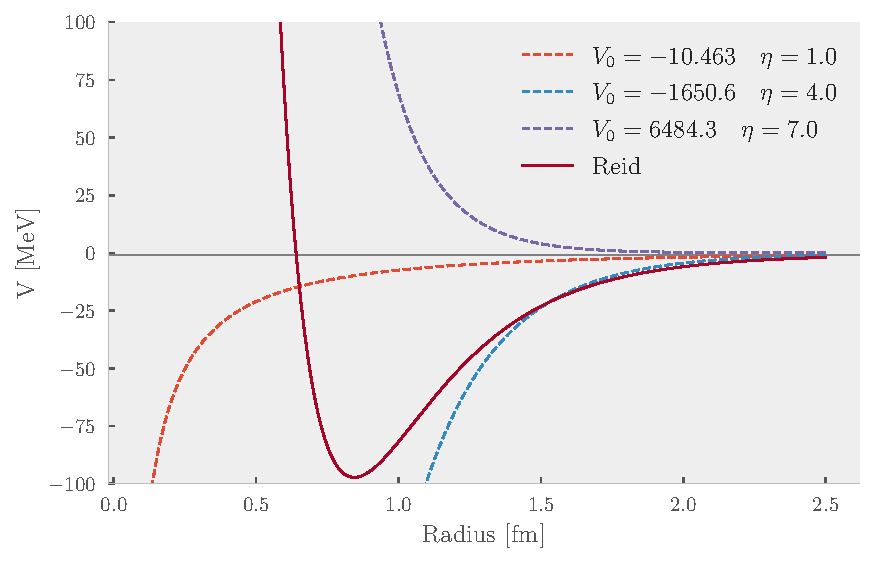
\includegraphics[]{Figures/reid.pdf}
  \caption{\label{fig:reid} The Reid potential (full stroke), a sum of three Yukawa potentials
  (dashed). It is has the typical characteristics of a nuclear force model, with
  a short range attractive potential followed by a repulsive core.}
\end{figure}

The Reid potential for \(np\) \(^{1}S_{0}\) was fit to several hundred data points
of the phase shift in the region \(0-350\) MeV, and thus should provide a good
fit in this region\cite{reid}.

% \begin{equation*}
%   V(\vec{r}) = \frac{f_{\pi}^{2}}{m_{\pi}^{2}}\left[ C_{\sigma}\sigma\cdot\sigma_{2} \right]
% \end{equation*}

% \begin{equation*}

%   V^{LO}(\vec{q}, \vec{k}) = C_{s} + C_{t}\vec{\sigma_{a}}\cdot\vec{\sigma_{2}}
% \end{equation*}

% \begin{equation*}
%   V^{NLO}(\vec{q}, \vec{k}) = C_{1}\vec{q}^{2} + C_{2}\vec{k}^{2} + \vec{\sigma}_{1}\cdot\vec{\sigma}_{2}
%   + iC_{5}\frac{\vec{\sigma}_{1}+\vec{\sigma}_{2}}{2}\cdot\vec{q}\times\vec{k}
%   + C_{6}\vec{q}\cdot\vec{\sigma}_{1}\vec{q}\cdot\vec{\sigma}_{2}
%   + C_{7}\vec{k}\cdot\vec{\sigma}_{1}\vec{k}\cdot\vec{\sigma}_{2}
% \end{equation*}

% where \(\vec{q} = \vec{p} - \vec{p}^{\prime}\) is the momentum transfer, \(\k =
% \frac{\vec{p}+\vec{p}^{\prime}}{2}\) the average momentum, and \(\vec{p}\) and
% \(\vec{p}^{\prime}\) the relative momenta.

\subsection{Fitting to Data}

The potential derived from EFT is incomplete, lacking values for its LECs that
must be obtained from comparison to experimental data. The potential itself is
unobservable \footnote{In fact, there is no reason to expect the EFT potential to converge to
  the ``true'' potential at all. EFT approximates the true high energy behavior
  by a simpler structure, reflected in the long range part of the EFT potential
  converging to the ``true'' potential while the short range part may deviate\cite[p.~17]{lepage1997renormalize}}
- instead one must use it to compute some other observable
quantities. There are no hard and fast rules for which observables to use,
common options being the scattering length and energy levels. Here we
will for simplicity's sake only use the \(^{1}S_{0}\) phase shift, at the cost
of accuracy and fitting robustness. 



%%% Local Variables:
%%% mode: latex
%%% TeX-master: "../main"
%%% TeX-engine: xetex
%%% End:
